\section{Vapour and Humidity}

\begin{multicols}{2}


\section*{Evaporation}


\subsection{Surface Area and Evaporation}

\begin{center}
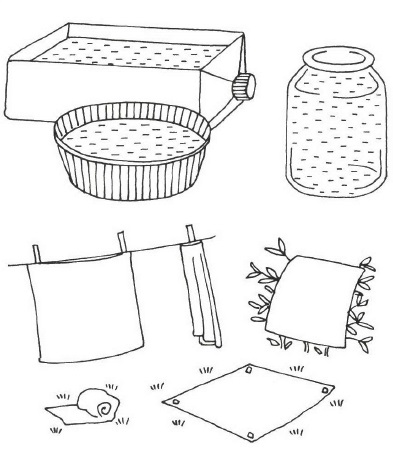
\includegraphics[width=0.4\textwidth]{./img/vso/sa-evaporation.jpg}
\end{center}

\begin{description*}
%\item[Subtopic:]{}
\item[Materials:]{Open containers of difference sizes, water}
%\item[Setup:]{}
\item[Procedure:]{Fill different containers with water and place them outside on a sunny day. Check the containers periodically to see which has lost the most water.}
%\item[Hazards:]{}
%\item[Questions:]{}
\item[Observations:]{Containers with a larger surface area lose more water due to evaporation.}
%\item[Theory:]{}
\item[Applications:]{This is why we spread out our clothes in the sun after washing them. The greater the surface area, the more quickly water evaporates.}
%\item[Notes:]{}
\end{description*}

%==================================================================================================%

\section*{Humidity}


\subsection{Relative Humidity}

\begin{center}
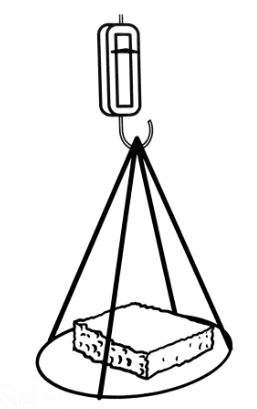
\includegraphics[width=0.25\textwidth]{./img/rel-humidity.jpg}
\end{center}

\begin{description*}
%\item[Subtopic:]{}
\item[Materials:]{Sponge, \nameref{sec:spring-balance}, \nameref{sec:scale-pan}}
%\item[Setup:]{}
\item[Procedure:]{Weigh a dry sponge using a spring balance. Then wet the sponge so it is soaked but not dripping and weigh again to determine the weight of water added. Dry the sponge again and add $^1/_2$ or $^1/_4$ of the water that the sponge can hold. }
%\item[Hazards:]{}
%\item[Questions:]{}
%\item[Observations:]{}
\item[Theory:]{The sponge represents the air. When soaked, it is said to be \emph{saturated}, i.e. it contains 100\% of the moisture it is capable of holding. When holding $^1/_2$ of that amount of water, it is 50\% saturated, and so on.}
%\item[Applications:]{}
%\item[Notes:]{}
\end{description*}

%\columnbreak

\subsection{The Hygrometer}

\begin{center}
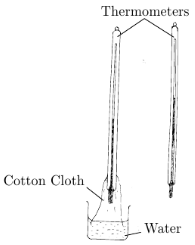
\includegraphics[width=0.4\textwidth]{./img/hygrometer.png}
\end{center}

\begin{description*}
%\item[Subtopic:]{}
\item[Materials:]{2 mercury or alcohol thermometers, container of water, cotton cloth, thread}
%\item[Setup:]{}
\item[Procedure:]{Wrap one of the thermometers with the cloth, tie it securely with string, and dip it into the water. Remove from the water and tie the tops of both thermometers with thread. Holding the thread tightly, quickly spin the thermometers together over your head for at least 30 seconds. Read and record the temperatures on both thermometers.}
%\item[Hazards:]{Be careful when spinning the thermometers. Make sure the string is strong enough to hold them and that there are no objects nearby to hit.}
%\item[Questions:]{}
\item[Observations:]{The reading on the thermometer with the cloth drops.}
\item[Theory:]{When rotated the cloth loses water and is therefore cooled by evaporation. The amount of water that the cloth loses depends on the humidity of the air. By observing the difference between the temperature of the wet cloth and air, we can tell the relative humidity (a small difference implies a high relative humidity and vice versa).}
%\item[Applications:]{}
%\item[Notes:]{}
\end{description*}

%==================================================================================================%


\end{multicols}

\pagebreak